\begin{doublespace}

\chapter{The role of standing genetic variation
  in adaptation to a new environment}
\label{chap:sgv}



\section{Introduction}



When a population adapts to a new environment,
beneficial alleles may appear as new mutations
or come from standing genetic variation \citep{bar08}.
%
Standing genetic variation refers to the presence
of alternative alleles at each genetic locus in a population.
%
Standing genetic variation may be maintained
in a population for several reasons \citep{har97};
e.g., alleles with little or no effect on fitness
may rise to moderate frequencies by random genetic drift.
%
Standing genetic variation may be a major source
of beneficial alleles in a new environment,
with two important implications for the dynamics of adaptation.
%
First, adaptation from standing genetic variation
should be faster than adaptation from new mutations
because beneficial alleles would be immediately available
and would be present at higher frequencies \citep{bar08}.
%
Second, the distribution of fitness effects of alleles
from standing genetic variation should be different
than that of new mutations because standing genetic variation
has been `pre-tested' by surviving previous generations
of selection against deleterious alleles \citep{bar08}.



Whether standing genetic variation is an important source
of beneficial alleles for adaptation is unknown.
%
Studies have employed three main approaches
to answer this question (reviewed in \citet{bar08}):
analysis of the signature of selection,
presence of the beneficial allele in the ancestral population,
and phylogenetic analysis for inferring the history of alleles.
%
These methods, however, are necessarily indirect
and each has their unique set of problems.
%
Of course, the ``surest way to determine
the source of beneficial alleles is to locate
the genes themselves and establish their histories'' \citep{bar08}.
%
In this study, I used digital organisms (see p.~\pageref{sec:avida})
to follow individual alleles through time
as populations adapted to a new environment,
and I determined whether beneficial alleles
appeared as new mutations or came from standing genetic variation.
%
I also tested whether adaptation from standing genetic variation
was faster than from new mutations
and whether the fitness effects of standing genetic variation
were different from those of new mutations.



\section{Standing genetic variation in digital organisms}



To generate a well-adapted, sexual population
with standing genetic variation prior to the environmental change,
I initialized an empty `world' with an organism
that could replicate but could not perform any tasks.
%
I set the world size to 10,000 cells
and the environment to reward for
the default nine tasks \citep{len99}.
%\emph{not}, \emph{nand}, \emph{and}, \emph{orn},
%\emph{or}, \emph{andn}, \emph{nor}, \emph{xor}, and \emph{equ}.
%
I set the copy mutation rate to 0.1 mutations
per genome per generation and,
to ensure homologous recombination,
I fixed the length of all genomes to 200 instructions
and turned off insertion and deletion mutations.
%
I let 50 such replicate populations evolve
for 500,000 updates%
---a measurement of time in Avida---%
which was about 42,000 generations.
%
I then picked a random population in which
the consensus sequence could perform all nine tasks
(35 out of the 50 could perform all nine tasks),
and I took a random sample of 1,000 individuals
from this population to serve as
the ancestral population before the environmental change.



To measure the amount of standing genetic variation
in the ancestral population,
I measured the heterozygosity of each locus of the population.
%
The heterozygosity of a locus is $H = 1 - \sum_{i = 1}^{k} p_i^{2}$,
where $k$ is the number of alleles segregating at that locus
and $p_i$ is the frequency of the $i$th allele \citep[p.~15]{gil04}.
%
Here I adopted the convention that a locus
is polymorphic (i.e., has standing genetic variation)
if its most common allele has a frequency $<$~0.95 \citep[p.~53]{har97}.
%
A locus that had standing genetic variation
would have a minimum heterozygosity of
$1 - (0.95^{2} + 0.05^{2}) = 0.095$.
%
Because there are 26 possible alleles (i.e., instructions)
per locus in digital organisms,
the maximum possible heterozygosity is approximately 0.9615.



I found substantial standing genetic variation
in the ancestral population (Figure~\ref{heterozygosity-plot}).
%
Of 200 loci, 125 (62.5\%) were polymorphic.
%
The heterozygosity of each locus ranged from 0.0 to 0.8859,
with a mean heterozygosity of 0.3781 (0.3334--0.4246, 95\% bootstrap CI).
%
For comparison, \citet{ste01} found in humans
that the heterozygosity of 313 genes
ranged from 0.012 to 0.929, with a mean of 0.534.
%
In natural populations of \emph{E. coli}, \citet{sel80} found
that the heterozygosity of 20 enzyme-encoding genes
ranged from 0.055 to 0.887, with a mean of 0.4718.
%
My results demonstrate that the ancestral population
exhibited levels of standing genetic variation
consistent with that observed in biological populations.
%
Furthermore, they support the claim that standing genetic variation
is a ubiquitous property of evolving genetic systems \citep{gib04,bar08}.



\begin{figure}[b!]
\begin{center}
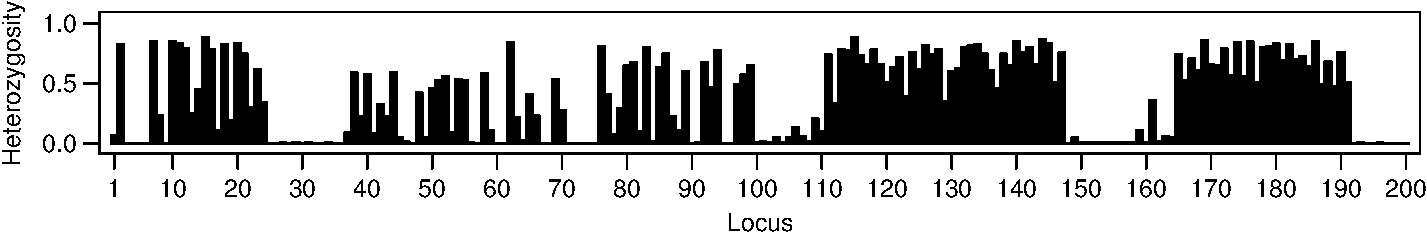
\includegraphics[width=\linewidth]{heterozygosity-plot.pdf}
\caption{The heterozygosity of each locus
  of the population before the environmental change.
  %
  Heterozygosities above 0.095 indicate
  the presence of standing genetic variation.}
\label{heterozygosity-plot}
\end{center}
\end{figure}



\section{Source of beneficial alleles}



Having established that the ancestral population
harbored abundant standing genetic variation,
I determined whether adaptation to a new environment
relied on this genetic variation or on new mutations
as a source of beneficial alleles.
%
In this study, I examined beneficial alleles
with fitness effects greater than 1\%.
%
With the ancestral population,
I started 20 new replicate populations
in a world of 1,000 cells and an environment
that rewarded for 68 different tasks
(the original nine tasks were not rewarded for).
%
As a control,
I also started another set of 20 replicate populations
where every individual had an identical genotype (i.e., isogenic),
set to the consensus sequence of the ancestral population.
%
Although the consensus genotype did not actually exist
in the ancestral population,
its fitness was 1.0070 relative to the highest fit individual
in the ancestral population
(excluding those who could immediately perform tasks),
and 1.0337 relative to the mean fitness of the ancestral population.
%
Thus, the control population was not at a disadvantage
compared to the ancestral population.
%
All other configuration settings were identical
to those used for the evolution of the ancestral population.
%
Note that the populations that started with standing genetic variation
were also allowed to get new mutations
(the mutation rate was set to 0.1 mutations per genome per generation).
%
I let these replicate populations
evolve for 10,000 updates ($\sim$~850 generations),
saving each population every 100 updates.





At the end of the runs, I found that
the populations that started with standing genetic variation
increased in mean fitness to 8.31 (7.74--8.87, 95\% bootstrap CI)
relative to the ancestral population in the new environment
(i.e., the evolved populations were 8.31 times
more fit in the new environment than the ancestral population).
%
These populations were able to perform
an average of 7.9 tasks, with a range of 5 to 10.
%
The mean number of fixed, derived alleles%
---defined as having a frequency $>$~0.95 in the evolved population
but $<$~0.95 in the ancestral population---%
was 56.25, ranging from 38 to 70.
%
Figure~\ref{allele-freq-plot} shows
the history of two allele fixation events,
one from standing genetic variation and the other from a new mutation,
that occurred in the first replicate population.
%
Of the 56.25 fixed, derived alleles,
47.8 (85\%) existed as standing genetic variation
in the ancestral population.
%
In the control populations, mean fitness increased
to 7.18 (6.62--7.76, 95\% bootstrap CI)
relative to the ancestral population.
%
The control populations were able to perform
an average of 6.7 tasks, with a range of 5 to 9.
%
The mean number of fixed, derived alleles
in the control populations was 5.15, ranging from 2 to 9.
%
It was surprising that the populations
that started with standing genetic variation
fixed 10 times more alleles than the control populations,
despite both sets of populations
having similar final fitnesses and
number of tasks performed.



\begin{figure}
\begin{center}
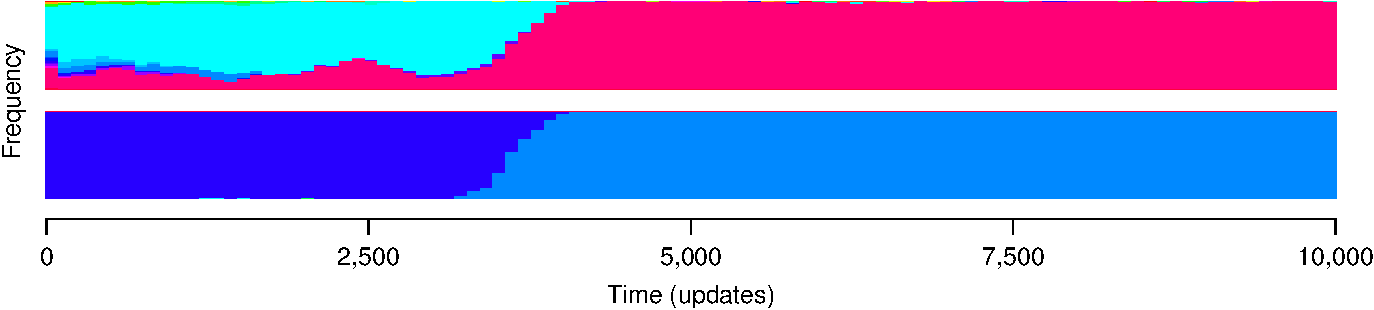
\includegraphics[width=\linewidth]{allele-freq-plot.pdf}
\caption{The frequencies of alleles through time for two loci
  in which an allele became beneficial and subsequently fixed.
  %
  In the top plot, the beneficial allele came from standing genetic variation,
  and in the bottom plot, the beneficial allele appeared as a new mutation.
  %
  Different alleles are represented by different colors.
  %
  The y-axis in each plot ranges from 0.0 to 1.0.
  %
  For interpretation of the references to color in this and all other figures, 
  the reader is referred to the electronic version of this dissertation.}
\label{allele-freq-plot}
\end{center}
\end{figure}



The finding that 85\% of fixed, derived alleles
in the populations that started with the ancestral population
existed as standing genetic variation
may indicate that most beneficial alleles came from standing genetic variation.
%
It is not clear, however, whether they were fixed
by neutral genetic drift, natural selection,
or genetic linkage and hitchhiking with beneficial alleles.
%
For example, genetic hitchhiking in Avida can occur
when alleles nearby a highly beneficial allele
rise in frequency along with the beneficial allele.
%
Hitchhiking occurs because the beneficial allele
and nearby (i.e., genetically linked) alleles
spread faster than recombination can break them apart.
%
It is also not clear at what frequency
the derived alleles first became beneficial.
%
Therefore, I developed a method to systematically
measure the fitness of individual alleles through time
and determine the frequency at which they became beneficial.





First, for each fixed, derived allele at the end of each run,
I calculated both the allele's frequency and fitness effect
every 100 updates, starting at the first update.
%
To calculate the fitness effect of an allele at the current update,
I first selected from the population the individual
with the highest fitness who had the allele.
%
I then created a clone of the individual and
substituted the allele with an alternative allele
drawn randomly from the standing genetic variation at that locus.
%
I then calculated the fitness of the individual with the allele
relative to the fitness of the individual without it.
%
If this relative fitness was greater than 1.01,
then the fitness effect of the allele ($>$~1\%)
was beneficial at the current update.
%
While testing this method, I found some cases where
the fitness effect of the allele was considered beneficial
only because the individual with the alternative allele
had unusually low fitness.
%
To reduce the frequency of such cases,
I also required that the allele be beneficial
for the individual with the second highest fitness.
%
I stopped analyzing further updates
as soon as I found the allele to be beneficial
or if it became fixed.


\begin{figure}[t!]
\begin{center}
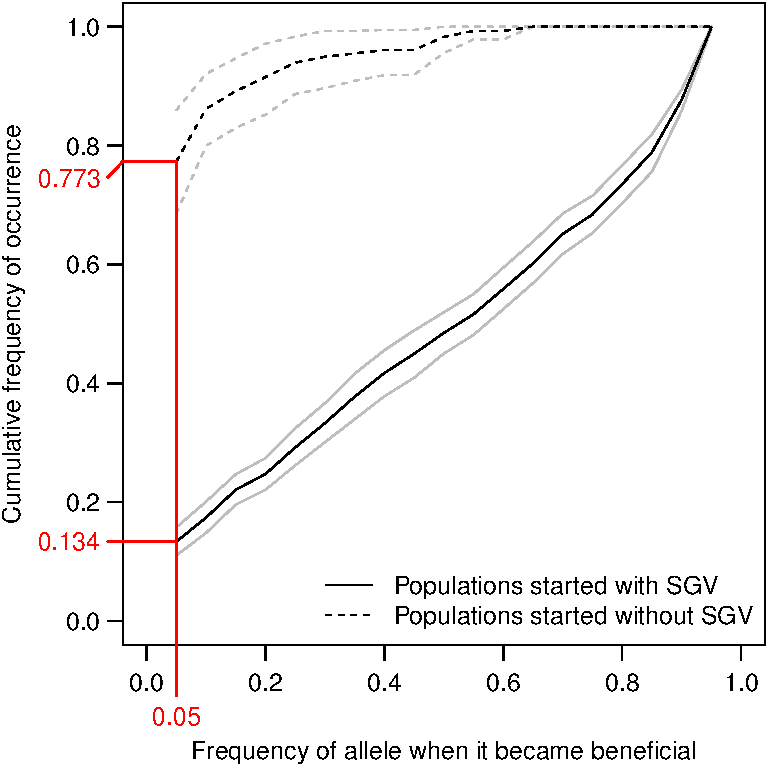
\includegraphics[width=3.5in]{cumul-freq-plot.pdf}
\caption{The cumulative frequency of fixed alleles
  that became beneficial at a specific frequency (0.05 bin size)
  for populations that started with standing genetic variation (solid lines)
  and for control, isogenic populations (dashed lines).
  %
  The gray lines indicate the 95\% bootstrap confidence interval
  around the mean of 20 replicate populations.
  %
  The red vertical line indicates the frequency
  below which alleles were considered to appear as new mutations.
  %
  The red horizontal lines indicate the proportions
  of alleles that came from new mutations
  for either type of population.}
\label{cumul-freq-plot}
\end{center}
\end{figure}


In populations that started with standing genetic variation,
I found that out of the mean 56.25 alleles that fixed,
a mean of 31.9 became beneficial at some point in their history.
%
I found that only 13.4\% of these beneficial alleles
became beneficial at a frequency $<$~0.05
(Figure~\ref{cumul-freq-plot}, lower horizontal red line);
the remaining 86.6\% became beneficial at a frequency $>$~0.05.
%
Supposing standing genetic variation comprises
alleles with frequencies $>$~0.05,
these results indicate that the majority of beneficial alleles
came from standing genetic variation.
%
In the control populations,
I found that out of the mean 5.15 alleles that fixed,
a mean of 5.1 became beneficial at some point in their history.
%
I found that 77.3\% of these beneficial alleles
became beneficial at a frequency $<$~0.05
(Figure~\ref{cumul-freq-plot}, upper horizontal red line);
the remaining 22.7\% became beneficial at a frequency $>$~0.05.
%
Therefore,
in contrast to populations that started with standing genetic variation,
the control, isogenic populations adapted mostly from new mutations,
although almost a quarter of beneficial alleles
came from standing genetic variation that arose
as populations accumulated genetic polymorphism over time.
%
Interestingly, the mean absolute (not percentage) number of new mutations
per replicate for each treatment was about the same:
4.15 (3.40--4.85, 95\% bootstrap CI) for populations started with
standing genetic variation and 3.75 (3.3--4.2) for isogenic populations.
%
This indicates that standing genetic variation did not
inhibit new mutations from being selected.





One potential concern with the above method
is that I identified beneficial alleles
based on only two genotypes that had the allele,
relative to two genotypes with alternative alleles.
%
Yet the presumed beneficial alleles as well as the alternative alleles
may not have the same fitness effect on other genetic backgrounds.
%
Thus, I implemented a second method to identify beneficial alleles
that considered more genotypes when measuring fitness effects.
%
The key difference between this method and the previous
is that in this method I selected all individuals who had the allele.
%
Then, for each of these individuals
I substituted the allele with an alternative allele
drawn randomly from the standing genetic variation at that locus.
%
Finally, I calculated the mean fitness of all individuals with the allele
relative to the mean fitness of all individuals with the allele replaced.
%
If this relative fitness was greater than 1.01,
then I considered the allele as beneficial.
%
Using this method, I found that
in populations that started with standing genetic variation,
11.5\% of alleles became beneficial at a frequency $<$~0.05;
the remaining 88.5\% became beneficial at a frequency $>$~0.05.
%
In the isogenic populations,
I found that 79.4\% of alleles became beneficial at a frequency $<$~0.05;
the remaining 20.6\% became beneficial at a frequency $>$~0.05.
%
These results are very similar to those I found with the previous method,
showing that the previous method was robust
to the number of genotypes considered when identifying beneficial alleles.



\section{Speed of adaptation}



Adaptation from standing genetic variation
should be faster than adaptation from new mutations
because beneficial alleles would be immediately available
and would be present at higher frequencies \citep{bar08}.
%
To test this prediction,
I compared the speed of adaptation between
populations that started with standing genetic variation
and those that started with isogenic individuals.
%
I re-evolved both types of populations
at the additional mutation rates (\emph{U})
of 0.01 and 0.0 (no new mutations) per genome per generation
(the original populations were run at a mutation rate of 0.1).
%
I added these new treatments because,
given that the only source of mutations
for the isogenic populations were new mutations,
the mutation rate would be an important variable
on the rate of adaptation.
%
Population size would also be an important variable
on the rate of adaptation,
but I did not investigate its effects in this study.



I found that at the 0.1 mutation rate,
the rate of adaptation for populations
that started with standing genetic variation
was significantly greater for most of the first four thousand updates
than isogenic populations,
then became less significantly so for the rest of the run
(Figure~\ref{pop-fitness-plot}A).
%
At the 0.01 mutation rate, however,
the rate of adaptation was significantly greater for the entire run
(Figure~\ref{pop-fitness-plot}B).
%
Interestingly, at the 0.0 mutation rate,
populations with standing genetic variation
continued to adapt for several thousand updates,
but, as expected, isogenic populations could not evolve
(Figure~\ref{pop-fitness-plot}C).
%
These results clearly demonstrate that
adaptation from standing genetic variation
was faster than from new mutations.
%
Yet new mutations were necessary for long-term evolution,
as shown by the fact that adaptation
from standing genetic variation without new mutations
stopped after several thousand updates.



\begin{figure}
\begin{center}
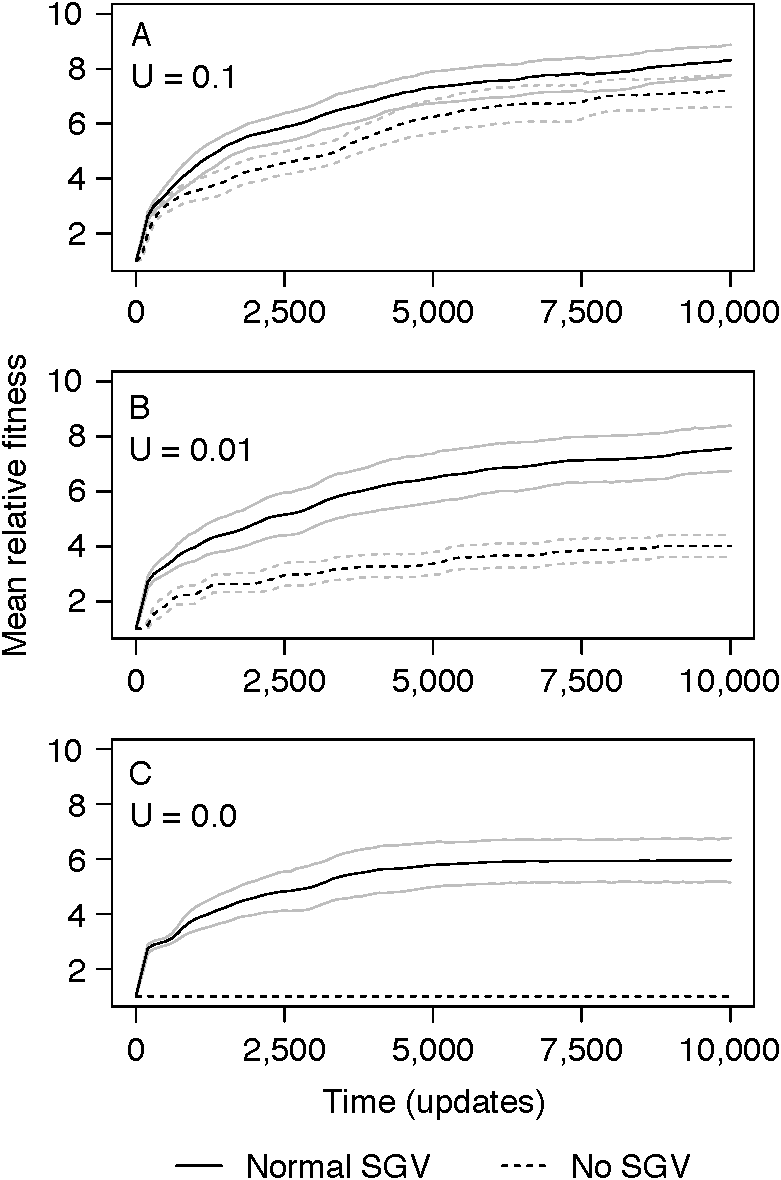
\includegraphics[width=4in]{pop-fitness-plot.pdf}
\caption{The mean fitnesses (relative to the ancestor)
  of populations evolved after an environmental change
  at (\textbf{A})~0.1, (\textbf{B})~0.01,
  and (\textbf{C})~0.0 mutations per genome per generation (\emph{U}).
  %
  Populations evolved starting either
  with the ancestral population (solid line),
  which contained standing genetic variation (SGV)
  or with an isogenic population based on
  the consensus sequence of the ancestral population (dashed line).
  %
  Gray lines represent the 95\% bootstrap confidence intervals
  around the mean.}
\label{pop-fitness-plot}
\end{center}
\end{figure}



\section{Fitness effect of random alleles from different sources of variation}

% - beneficial/fixed allele is present in ancestral population
%   - what was its frequency in ancestral pop?
%   - what was its effect in ancestral pop (e.g., neutral, deleterious)?
% - beneficial allele has been pre-tested:
%   - increases chance that fitness effect is advantageous

%Standing genetic variation is often
%maintained by the neutrality of alleles
%in the ancestral environment \citep{bar08}.
%%
%To test this,
%I measured the fitness of the beneficial alleles
%in standing genetic variation
%identified above in the ancestral environment.
%%
%I found that across all replicates only about 5\%
%of fitness effects were under 0.99,
%and the mean was 0.9936 (0.9847--1.003, 95\% bootstrap CI).


The distribution of fitness effects of alleles
from standing genetic variation should be different
than that of new mutations because standing genetic variation
has been `pre-tested' by selection \citep{bar08}.
%
To test this prediction,
I generated the fitness effect distribution
of alleles coming from either standing genetic variation
or new mutations, measured in the new environment.
%
First, I sampled 1,000 random (but viable)
individuals from the ancestral population
and mutated a single, random locus of each individual
to an allele drawn randomly from the standing genetic variation
(if there was any variation at that locus).
%
I also sampled another set of 1,000
individuals from the ancestral population
and mutated a single locus of each individual
to an allele drawn randomly from all 25 possible alternative alleles.
%
To prevent the possibility that these random mutations
were more deleterious only because they disrupted fixed alleles,
I ensured that the loci were drawn from the same pool
of loci that had standing genetic variation.
%
Finally, I measured the fitness of these mutants
relative to the original, unmutated individual.



I found that the mean fitness of mutants
with mutations from standing genetic variation
was 0.9994 (0.9969--1.0023, 95\% bootstrap CI).
%
The mean fitness of mutants with random mutations
was 0.9496 (0.9326--0.9665, 95\% bootstrap CI).
%
Clearly, mutations from standing genetic variation
did not have, on average, as strong deleterious effects
as random mutations.
%
To examine more closely the fitness effects
of mutations from the two sources,
I categorized each mutation based on
the mutant's relative fitness (Table~\ref{mutant_fitness_table}).
%
Alleles from standing genetic variation were mostly neutral,
whereas new mutations were more likely to be lethal or deleterious.
%
Interestingly, new mutations were also more likely
to be strongly beneficial than alleles from standing genetic variation,
yet in the analysis where I determined the source of beneficial alleles,
I found that most beneficial alleles came from standing genetic variation.
%
This discrepancy may indicate that although alleles
from standing genetic variation were not beneficial alone,
combinations of these alleles brought together
by recombination provided the benefits.
%
The finding that alleles from standing genetic variation
were less deleterious on average than random mutations
support the hypothesis that standing genetic variation
has been pre-tested by selection.



\begin{table}
\begin{center}
\begin{tabular}{lcc}
\cline{2-3}
\multicolumn{1}{l}{} & \multicolumn{2}{c}{Source of mutation} \\
\hline
Fitness effect & SGV & Random \\
\hline
Lethal & 0 & 58 \\
Strongly deleterious & 3 & 5 \\
Mildly deleterious & 186 & 345 \\
Nearly neutral & 729 & 520 \\
Mildly beneficial & 81 & 67 \\
Strongly beneficial & 1 & 5 \\
\hline
\end{tabular}
\caption{The number of single mutants (out of 1,000),
  categorized by the mutation's source and fitness effect ($w$):
  lethal ($w =$~0),
  strongly deleterious (0~$< w \le$~0.99),
  mildly deleterious (0.99~$< w \le$~0.999),
  neutral or nearly neutral (0.999~$<$ $w \le$~1.001),
  mildly beneficial (1.001~$< w \le$~1.01),
  and strongly beneficial ($w >$~1.01).}
\label{mutant_fitness_table}
\end{center}
\end{table}



The above analysis was based on randomly generated mutants
of the ancestral genotypes (i.e., at the beginning of the experiments),
but it would also be interesting to know
the fitness effect of beneficial alleles that actually fixed.
%
This information was already calculated
as part of determining the moment at which alleles
became beneficial because it was used to determine
whether alleles had achieved a fitness $>$~1.01 (using the first method).
%
For populations that had evolved under standing genetic variation,
the mean fitness of a genotype with a beneficial allele
at the moment at which it became beneficial
(relative to a genotype without the beneficial allele)
was 1.54 (1.48--1.60, 95\% bootstrap CI).
%
For isogenic populations,
this mean fitness was 1.47 (1.37--1.59, 95\% bootstrap CI).
%
Although the mean fitness effect of beneficial alleles
for the standing genetic variation treatment
was slightly higher than the isogenic treatment,
they were not significantly different.
%
The maximum relative fitness for a genotype with a beneficial allele
for the standing genetic variation treatment (7.05)
was higher than that for the isogenic treatment (4.50).





\section{Discussion}


% every statement I make must be supported by my results,
% the results of others, or authoritative statements
% based on the results of others
% - the reference must be the one from which the original
%   information came, not from a paper that used that information
%   to make further arguments

% Start with the main point: source of beneficial mutations,
% using the same words I used in the Introduction


I have shown that in populations of digital organisms
adapting to a new environment,
the major source of beneficial alleles
was standing genetic variation, not new mutations.
%
My findings are supported by
selection experiments and observational studies
of biological populations.
%
Selection experiments have shown that
adaptation can occur by changes in allele frequencies
of standing genetic variation in the initial populations
\citep[e.g.,][]{fed97,sca09,teo09}.
%
Observational studies of natural populations
have found that alleles correlated with adaptive traits
were also present in the ancestral population
\citep[e.g.,][]{col05,myl05}.
%
% (Examples of new mutations?)
%
In biological organisms, however,
it is very difficult to measure
the fitness effects of individual alleles,
which is necessary to determine whether
an allele fixed due to selection.
%
Another problem, specific to studies of natural populations,
is that the ancestral population is unavailable%
---the closest one can get is the extant population
from which a subpopulation founded a new environment---%
and therefore it is often unknown
whether a beneficial allele existed as standing genetic variation.
%
The use of digital organisms allowed me to track
individual alleles through time
and determine the frequency at which they became beneficial.

% Something about generalization
%I show that in a general evolving genetic system,
%standing genetic variation provides most of the beneficial alleles
%to a population adapting to a new environment.



When alleles from standing genetic variation became beneficial,
their starting frequency ranged from the minimum of 5\%
to the maximum of 95\% (Figure~\ref{cumul-freq-plot}).
%
In experimental studies of biological organisms,
high starting frequencies ($>$~50\%) are not uncommon
\citep[e.g.,][]{fed97,sca09}.
%
In natural populations, however,
starting frequencies have tended to be much smaller,
such as in the study by \citet{col05},
where the starting frequency of an adaptive allele
was between 0.2\% and 3.8\% in the ancestral population.
%
One possible reason for this discrepancy
is that natural populations may be under stronger selective pressures
than experimental populations \citep{ell08},
so the fitness effects of alleles in natural populations
tend to be more deleterious and therefore maintained at low frequencies.
%
Of course, allele frequency data for adaptive alleles
in natural populations is scarce,
so more research in natural populations
should determine the frequencies at which alleles
from standing genetic variation become beneficial.



Adaptation should be faster if most beneficial alleles
came from standing genetic variation
than if they came from new mutations \citep{bar08}.
%
I found this to be the case in digital organisms
if the mutation rate was low enough (Figure~\ref{pop-fitness-plot}).
%
In fact, when no new mutations were allowed,
adaptation by standing genetic variation continued
for several hundred generations,
whereas no adaptation occurred in isogenic populations.
%
Still, the importance of new mutations
for long-term evolution was shown by the fact
that adaptation stopped eventually
when no new mutations were allowed.
%
Although there are no empirical studies
testing the speeds of adaptation,
where beneficial alleles may come from
either standing genetic variation or new mutations,
my results are supported theoretically \citep{her05}.
%
There are two reasons that adaptation
from standing genetic variation should be faster
than adaptation from new mutations:
beneficial alleles are both readily available
and present at higher frequencies than alleles
from new mutations \citep{bar08},
which must overcome drift because they start at lower frequencies.
%
Future experiments should be able to quantify
the relative contribution of these two causes.



Although not examined in detail in this study,
the population size and mutation rate can affect the relative contributions
of standing genetic variation and new mutations during adaptation.
%
For example, a sudden decrease in population size (i.e., a bottleneck)
will reduce both the amount of standing genetic variation
and the number of new mutations that appear each generation.
%
In this case, standing genetic variation
will still have an advantage over new mutations---%
especially for alleles of weak fitness effect---%
because weak effect alleles introduced by new mutations
are easily lost due to genetic drift \citep{her05}.
%
For large effect alleles,
standing genetic variation will have a reduced advantage
because large effect alleles are less likely to be lost
even if they are introduced as new mutations \citep{her05}.
%
In my experiments, mutations that allowed organisms
to perform new tasks were of large effect
(the default configuration in Avida),
but future studies should experiment with weaker beneficial alleles.
%
In a large population or high mutation rate,
new mutations would become more important
because large-effect mutations would appear more frequently.



Because alleles from standing genetic variation
have had a potentially long history in an evolving population,
their fitness effects in a new environment
have been predicted to be less deleterious
than random mutations \citep{bar08}.
%
On average, I found that
standing genetic variation was effectively neutral
(fitness effect of 0.0006),
whereas random mutations were strongly deleterious
(fitness effect of 0.0504).
%
Alleles from standing genetic variation can therefore linger in a population,
increasing the chance for them to become beneficial
after an environmental or genetic change.
%
Random mutations, on the other hand, are on average deleterious
and are thus more easily eliminated by selection.
%
In biological populations,
the mean fitness effect of random mutations
was found to be 0.48 in RNA viruses \citep{san04},
0.12 in \emph{C. elegans} \citep{vas00},
and 0.22 in yeast \citep{zey01}.
%
There are no measurements of the fitness effects
of alleles from standing genetic variation
in a biological population in a new environment.



For strongly beneficial mutations (i.e., fitness effect $>$~1\%),
I found that random mutations were more likely to be beneficial
than alleles from standing genetic variation
in the new environment (Table~\ref{mutant_fitness_table}).
%
It may thus seem counter-intuitive that
most beneficial alleles during adaptation
came from standing genetic variation.
%
I hypothesize that it was the combination of many alleles
from standing genetic variation that provided the benefits,
and together these epistatically related alleles rose to fixation.
%
Adaptation that requires many alleles working together
is known as `polygenic adaptation' \citep{pri10},
although fixation of alleles is not always necessary.
%
In fact, \citet{pri10} hypothesize that if
adaptation occurs from standing genetic variation,
polygenic adaptation is likely.



In summary,
this study has shown the importance of standing genetic variation
in populations of digital organisms adapting to a new environment.
%
That is,
(1) most beneficial alleles came from standing genetic variation
rather than from new mutations,
(2) populations that started with standing genetic variation
adapted faster than populations that started with identical genotypes,
and (3) the fitness effects of alleles from standing genetic variation
were less harmful than new mutations.
%
Because digital organisms evolve by the same
processes of natural selection and genetic drift
that biological populations also experience,
I suspect that the above points are also true for biological populations.
%
A hypothesis that arose from this study
was that standing genetic variation together with recombination
may give rise to combinations of alleles that together are beneficial.
%
Future work should test whether this additional advantage is true,
thereby highlighting the importance of sexual recombination
and standing genetic variation in evolving populations.


% consider plotting the substitutions through time

% paragraph on limitations of Avida

% paragraph on future work

% say something about cryptic genetic variation

% undoubtedly, more loci are important (not just fixed),
% as has been observed in literature, but fixed gave us a starting point

% Colosimo et al - Eda: 0.2% and 3.8%

% FRIGIDA - 40% - 60% (artificial)

% Feder et al 1997:
% hawthorns are the ancestral host of R. pomonella
% - so hawthorn race of pomonella is ancestral pop of apple pomonella?

% Teotonio: 70% of SNPs had freqs > 5% in control/ancestral pops
% - allele frequencies didn't change much although adaptation occurred

% Begin with I found and THEN compare them to other studies

% Always end with a conclusion, something drawn out of my results,
% but a conclusion can be a summary of the issue incorporating my findings,
% a recommendation, speculation (that could be used to form a new hypothesis),
% a new principle, or that there isn't enough evidence to form a conclusion
% - the conclusion should be a simple, easy to read sentence

% ideas developed from the results
% practical application or contribution to general thinking of my discipline

% start paragraphs with a brief summary of what's to come,
% and include a transition from the previous paragraph

% organize ideas in order of importance
% 1 - relevant to original hypothesis, accept/reject
% 2 - relevant, but not conclusive; need more study
% 3 - not relevant to original hypo, but based on results; new & interesting
% 4 - anything else -- excise from discussion

% What are the limitations of my study?

% What remains to be done, suggest additional research
% What more would I like to know?

% Why is my claim significant?
% What are its consequences?
% Any new significance not mentioned in the Intro?
% (but careful not to make it the main point)



% Things to consider:

% New mutations have to be important for long-term evolution
% - it could be that mutations serve to generate SGV,
%   but evolution mostly happens from SGV
%   - would have to track where mutations come from
%     in the mutation-only treatment

% I find that ANOTHER reason sgv is good for adaptation
% is that beneficial COMBINATION of alleles are already present,
% whereas mutation typically happens one-by-one

% Future work: How does sgv change through time
%   for those that started with sgv and those that didn't.

% Future work: more generations, long-term

\end{doublespace}

\begin{lit_cited}
\end{lit_cited}
\addcontentsline{toc}{section}{LITERATURE CITED}

% Temporarily remove section number from bibliography title
\renewcommand\bibsection{\center\section*{\bibname}}

\bibliographystyle{apalike}
\bibliography{sgv}

\renewcommand\bibsection{\section{\bibname}}
